\documentclass[10pt, titlepage, oneside, a4paper]{article}
\usepackage[swedish]{babel}
\usepackage[T1]{fontenc}
\usepackage[titletoc]{appendix}
\usepackage[utf8]{inputenc}
\usepackage{amssymb, graphicx, fancyhdr}
\usepackage{amsmath}
\usepackage{amsthm,algorithm,algorithmic,yhmath,enumitem,lscape}
\usepackage{float}
\usepackage{hyperref, url}
\usepackage{minted}

\newmintinline{c}{}

\addtolength{\textheight}{20mm}
\addtolength{\voffset}{-5mm}
\renewcommand{\sectionmark}[1]{\markleft{#1}}

\def\inst{datavetenskap}
\def\typeofdoc{Obligatorisk uppgift 1}
\def\course{5DV149 Datastrukturer och algoritmer}
\def\pretitle{Pretitle}
\def\title{Obligatorisk uppgift 1 --- Testning av stack}
\def\name{Name}
\def\username{CS username}
\def\email{\musername{}@cs.umu.se}
\def\graders{Graders}

\def\mfullpath{\raisebox{1pt}{$\scriptstyle \sim$}\musername/\path}
\def\nfullpath{\raisebox{1pt}{$\scriptstyle \sim$}\nusername/\path}

\newcommand{\R}{\mathbb{R}}
\newcommand{\N}{\mathbb{N}}
\newcommand{\Rn}{\mathbb{R}^n}
\newcommand{\Rnn}{\mathbb{R}^{n \times n}}
\newcommand{\bes}{\begin{equation*}}
\newcommand{\ees}{\end{equation*}}
\newcommand{\be}{\begin{equation}}
\newcommand{\ee}{\end{equation}}
\newcommand{\bms}{\begin{multline*}}
\newcommand{\emults}{\end{multline*}}
\newcommand{\bbm}{\begin{bmatrix}}
\newcommand{\ebm}{\end{bmatrix}}
\newcommand{\eps}{\epsilon}
\newcommand{\fl}{\text{fl}}
\newcommand{\Lp}{{L^p}}
\newcommand{\Ker}{\text{Ker}\,}
\newcommand{\loc}{{\text{loc}}}
\newcommand{\ccinf}{C_c^\infty}
\newcommand{\supp}{\text{supp}}
\newcommand{\dist}{\text{dist}}

\begin{document}
	\begin{titlepage}
		\thispagestyle{empty}
		\begin{large}
			\begin{tabular}{@{}p{\textwidth}@{}}
				\textbf{UMEÅ UNIVERSITET \hfill \today} \\
				\textbf{Institutionen för \inst} \\
				\textbf{\typeofdoc} \\
			\end{tabular}
		\end{large}
		\vspace{25mm}
		\begin{center}
			\LARGE{\pretitle} \\
			\huge{\textbf{\course}}\\
			\vspace{10mm}
			\LARGE{\title} \\
			\vspace{15mm}
            \LARGE{version 1.0} \\
            \vspace{10mm}
			\begin{large}
				\begin{tabular}{ll}
					\textbf{Namn} & \name \\
					\textbf{Användarnamn} & \username \\
				\end{tabular}
			\end{large}
			\vfill
            \vfill
			\large{\textbf{Labrättare}}\\
			\mbox{\large{\graders}}
		\end{center}
	\end{titlepage}
    
    % fixar sidfot
	\lfoot{\footnotesize{\name, \username}}
	\rfoot{\footnotesize{\today}}
	\lhead{\sc\footnotesize\title}
	\rhead{\nouppercase{\sc\footnotesize\leftmark}}
	\pagestyle{fancy}
	\renewcommand{\headrulewidth}{0.2pt}
	\renewcommand{\footrulewidth}{0.2pt}

	% skapar innehållsförteckning.
	% Tänk på att köra latex 2ggr för att uppdatera allt
	\pagenumbering{roman}
	\tableofcontents
	% och lägger in en sidbrytning
	\newpage

	\pagenumbering{arabic}

	% i Sverige har vi normalt inget indrag vid nytt stycke
	\setlength{\parindent}{0pt}
	% men däremot lite mellanrum
	\setlength{\parskip}{10pt}

\section{Introduktion}

Skriv en kort introduktion till din rapport. I denna laboration räcker
det med kanske ett eller två stycken då målgruppen för din rapport är
handledarna och dom förväntas vara väl förtrogna med uppgiften och den
aktuella datatypen.

Viktigt! Om du väljer att ladda ner detta dokument och kompilera det
på din dator, använd kommandot
\begin{verbatim}
pdflatex -shell-escape rapport.tex
\end{verbatim}
Kom ihåg att köra kommandot två gånger för att uppdatera
innehållsförteckning, figurreferenser, osv.

\section{Gränsyta till datatypen Stack}

Beskriv gränsytan till datatypen Stack. Beskrivningen ska vara
strukturerad, men du får själv bestämma hur, t.ex. en undersektion per
funktion, en punktlista, en tabell med funktionerna, e.dyl.

I din beskrivning, utgå helst från det som är publicerad i
\texttt{stack.h} eller \texttt{int\_stack.h}. Som ett alternativ får
du välja en beskrivning som motsvarar den informella specifikationen
av datatypen från boken och föreläsningsanteckningarn.\footnote{Denna
möjlighet kommer att tas bort i framtida kurser. Den finns kvar endast
då det var tillåtet i den ursprungliga specifikationen.}

Du kommer att behöva skriva en liten beskrivning av skillnaden mellan
hur \cinline{stack} och \cinline{int_stack} är implementerade, men i
övrigt bör du undvika att kommentera vad du vet om hur datatypen är
implementerad.

Det viktiga är att det ska vara \textit{lätt att läsa} din
beskrivning. Exempelvis ska eventuell kod som du skriver bland löptext
ha annat ett \textbf{fixt typsnitt}, vilket går att lösa med
\texttt{Empty()} eller \cinline{Empty()}. I icke-\LaTeX-system kan du
använda typsnittet \texttt{Courier}.

Nedan skriver jag några \textit{exempel} för att visa på några tekniska
lösningar i Latex och Overleaf.

\begin{itemize}
\item \textbf{Empty()} --- Returnera en tom stack
\item \textbf{Push(s, v)} --- Stoppar värdet \textbf{v} överst på
  stacken \textbf{s} och returnerar den modifierade stacken.
\end{itemize}

\begin{center}
\begin{tabular}{l|l}
  \cinline{stack_empty(free)} & Returnerar en tom stack.\\\hline
  \cinline{stack_push(s, v)} & \parbox[t]{8cm}{Stoppar värdet \texttt{v} överst på stacken \texttt{s}
                               och returnerar det modifierade stacken.}
\end{tabular}
\end{center}

\subsection{\texttt{stack\_empty()}}

\begin{minted}[frame=single]{c}
  stack *stack_empty(free_function free_func);
\end{minted}

Funktionen \cinline{stack_empty(free)} returnerar en tom stack där
stacken har övertagit ansvaret för att avallokera elementvärden som
läggs på stacken.

\subsection{\texttt{stack\_push()}}

\begin{minted}[frame=single]{c}
  stack *stack_push(stack *s, void *v);
\end{minted}

Funktionen \cinline{stack_push(s, v)} placerar pekaren \texttt{v}
överst på stacken \texttt{s} och returnerar den modifierade
stacken. Ansvaret för att avallokera \texttt{v} övertas av stacken.

\subsection{more commands...}

\section{Dokumentation av testerna}

Det här är den viktigaste delen! Skriv några korta ord kring varje
test, vad du förutsätter ska fungera (redan testat av tidigare tester)
och hur du har tänkt kring testet. Undvik att använda kod i din
beskrivning --- det blir bara svårläst! Skriv t.ex. ``Testet lägger
ett element på en tom stack och kollar att stacken inte är tom'' eller
``testet placerar fyra värden på stacken och kontrollerar att dom
hamnar i rätt ordning''. (Plus fler detaljer om vilka funktioner du
anropar i vilken ordning och vad det förväntade resultatet är.)

\subsection{\cinline{int_stack}}

\subsubsection{Test 1 - namn}

\subsubsection{Test 2 - namn}

\subsection{\cinline{stack}}

\subsubsection{Test 1 - namn}

\subsubsection{Test 2 - namn}

\section{Resultat}

Specifikationen kräver två körningar: en på en korrekt stack och en på
en trasig stack. Skriv lite om dom här och referera t.ex. till
skärmdumpar som den i Figur~\ref{fig:ok-run}. Kom ihåg att skriva en
summering i löptexten också!

\begin{figure}
  \begin{center}
    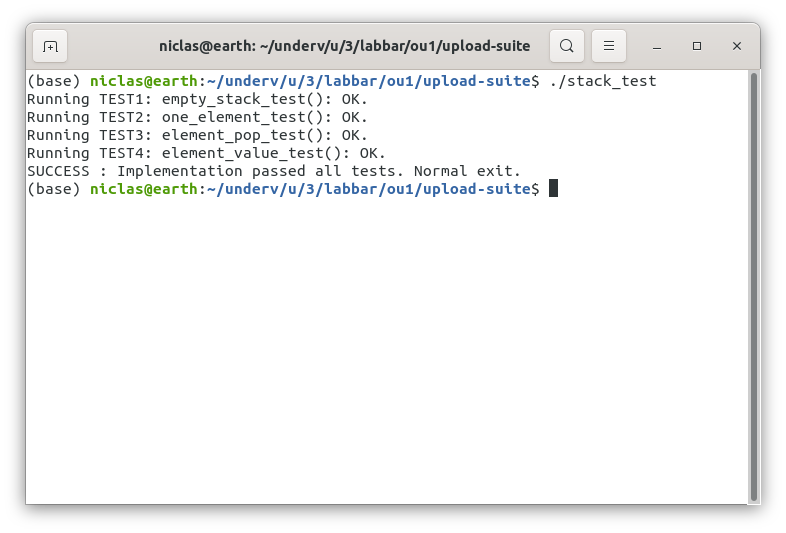
\includegraphics[width=0.6\hsize]{screendump-ok.png}
  \end{center}
  \caption{Testkörning 1. Testkörning mot en korrekt
    stack-implementation. Utskrifterna visar att koden klarade alla
    testerna.}
  \label{fig:ok-run}
\end{figure}

\end{document}
